\documentclass{beamer}
\usetheme{Antibes}
\usepackage[UTF8,scheme=plain]{ctex}
\usepackage{amsmath}
\usepackage{amsfonts}
\usepackage{amssymb}
\usepackage{mathrsfs}
\usepackage{bm}
\usepackage{graphicx}
\usepackage{float}
\usepackage{subfigure}
%\usepackage{biblatex}
\newcommand{\dif}{\mathop{}\!\mathrm{d}}

\title{Measurement of the absolute branching fraction of the inclusive semileptonic $\Lambda_c^+$ decay}
\author{严启宇,黄吉鸿,卢玫澍}
\institute{UCAS}
\date{2019/7/25}

\begin{document}
\bibliographystyle{IEEEtran}
\begin{frame}
    \titlepage
\end{frame}

\begin{frame}
    \frametitle{Outline}
    \tableofcontents
\end{frame}

\section{Overview}
\subsection{about$\Lambda_c^+$}
\begin{frame}
    \sectionpage
\end{frame}

\begin{frame}
    The lowest-lying charmed baryon $\Lambda_c^+$ was discovered more than 40 years ago\cite{knapp1976observation}\cite{abrams1980observation} , but its
    decays have not yet been fully mapped out due to the many available modes (about 80 kinds according to PDG2018). \\ 
    \vspace{0.2in}
    BESIII collaboration measured the absolute branching fraction of $\Lambda_c^+ \rightarrow \Lambda e^+ \nu_e$ to be $(3.63 \pm 0.43)\%$ \cite{ablikim2015measurement}.
    compared with the absolute branching fraction of $\Lambda_c^+ \rightarrow X e^+ \nu_e$ measured by MARK II as $(4.5 \pm 1.7)\%$.\cite{vella1982observation}

\end{frame}
\subsection{About this research}
\begin{frame}
    This research \cite{ablikim2018measurement} aims to measure the the absolute branching fraction of $\Lambda_c^+ \rightarrow X e^+ \nu_e$ more precisely, and to determine 
    the inclusive semileptonic decay widths $\frac{\Gamma(\Lambda_c^+ \rightarrow X e^+ \nu_e)}{\bar{\Gamma}(D\rightarrow X e^+ \nu_e)}$.\\
    \vspace{0.2in}
    And the result is: $\mathcal{B}(\Lambda_c^+ \rightarrow X e^+ \nu_e) = (3.95\pm0.34\pm0.09)\%$ \\ $\frac{\Gamma(\Lambda_c^+ \rightarrow X e^+ \nu_e)}{\bar{\Gamma}(D\rightarrow X e^+ \nu_e)}=1.26\pm0.12$
\end{frame}

\subsection{What does the result tell us}
\begin{frame}
    $\mathcal{B}(\Lambda_c^+ \rightarrow X e^+ \nu_e) = (3.95\pm0.34\pm0.09)\%$: center value is larger than that of $\mathcal{B}(\Lambda_c^+ \rightarrow \Lambda e^+ \nu_e)=(3.63 \pm 0.43)\%$. But it's difference is less than $1\sigma$.
    It is difficult to determine if there is other kinds of semileptonic decay. if there is, its absolute branching fraction will be much smaller than that of $\Lambda_c^+ \rightarrow X e^+ \nu_e$\\
    \vspace{0.2in}
    $\frac{\Gamma(\Lambda_c^+ \rightarrow X e^+ \nu_e)}{\bar{\Gamma}(D\rightarrow X e^+ \nu_e)}=1.26\pm0.12$: This ratio is predicted to be $1.67$ using an effective-quark theory calculation. \cite{gronau2011ratios} and 1.2 based on a calculation using the heavy-quark expansion \cite{manohar1994inclusive}.
    A more precise measurement is needed to verify those theory.
\end{frame}

\section{About this experiment}
\begin{frame}
    This research used a double-tag method to obtain the branching fraction of the inclusive semileptonic $\Lambda_c^+$ decay. \\
    \vspace{0.2in}
    And used a common way to choose vaild track, filter by invariant mass and beam energy, linear correction for particle identification (PID) and "Right Sign-Wrong Sign" method.
\end{frame}

\subsection{Double Tag}
\subsubsection{Tagging $\bar{\Lambda}_c^-$}
\begin{frame}
    We can tell from symmetry, when electron and positron annihilations, they creates matter and antimatter. Then matter and antimatter dacays, not affected by each other. The branching fraction should be the same among them.\\
    \vspace{0.2in}
    When it comes to $\Lambda_c^+$ and $\bar{\Lambda}_c^-$, $e^+e^-\rightarrow \Lambda_c^+\bar{\Lambda}_c^-$ is the process that produces $\Lambda_c^\pm$. \\
    \vspace{0.2in}
    It is difficult to figure out how many $\Lambda_c^+\bar{\Lambda}_c^-$ pairs are produces in an experiment. But due to the decay of $\Lambda_c^+$ and $\bar{\Lambda}_c^-$ are independent (statistically independent):\\
    \vspace{0.2in}
    We always have : $\Pr(A\mid B)=\Pr(A)$, where "A" means $\Lambda_c^+$ decays into $X e^+ \nu_e$ and "B" means $\bar{\Lambda}_c^-$ decays into $\bar{p} K^0_S$ or $\bar{p} K^+ \pi^-$, which have a low background and easy to reconstruct.
\end{frame}

\begin{frame}
    That is the mathematical way to explain Double-Tag in this experiment. When doing the data analysis. We first fully reconstruct one $\bar{\Lambda}_c^-$. (Effiency is about $58\%$)
    \begin{figure}
        \centering
        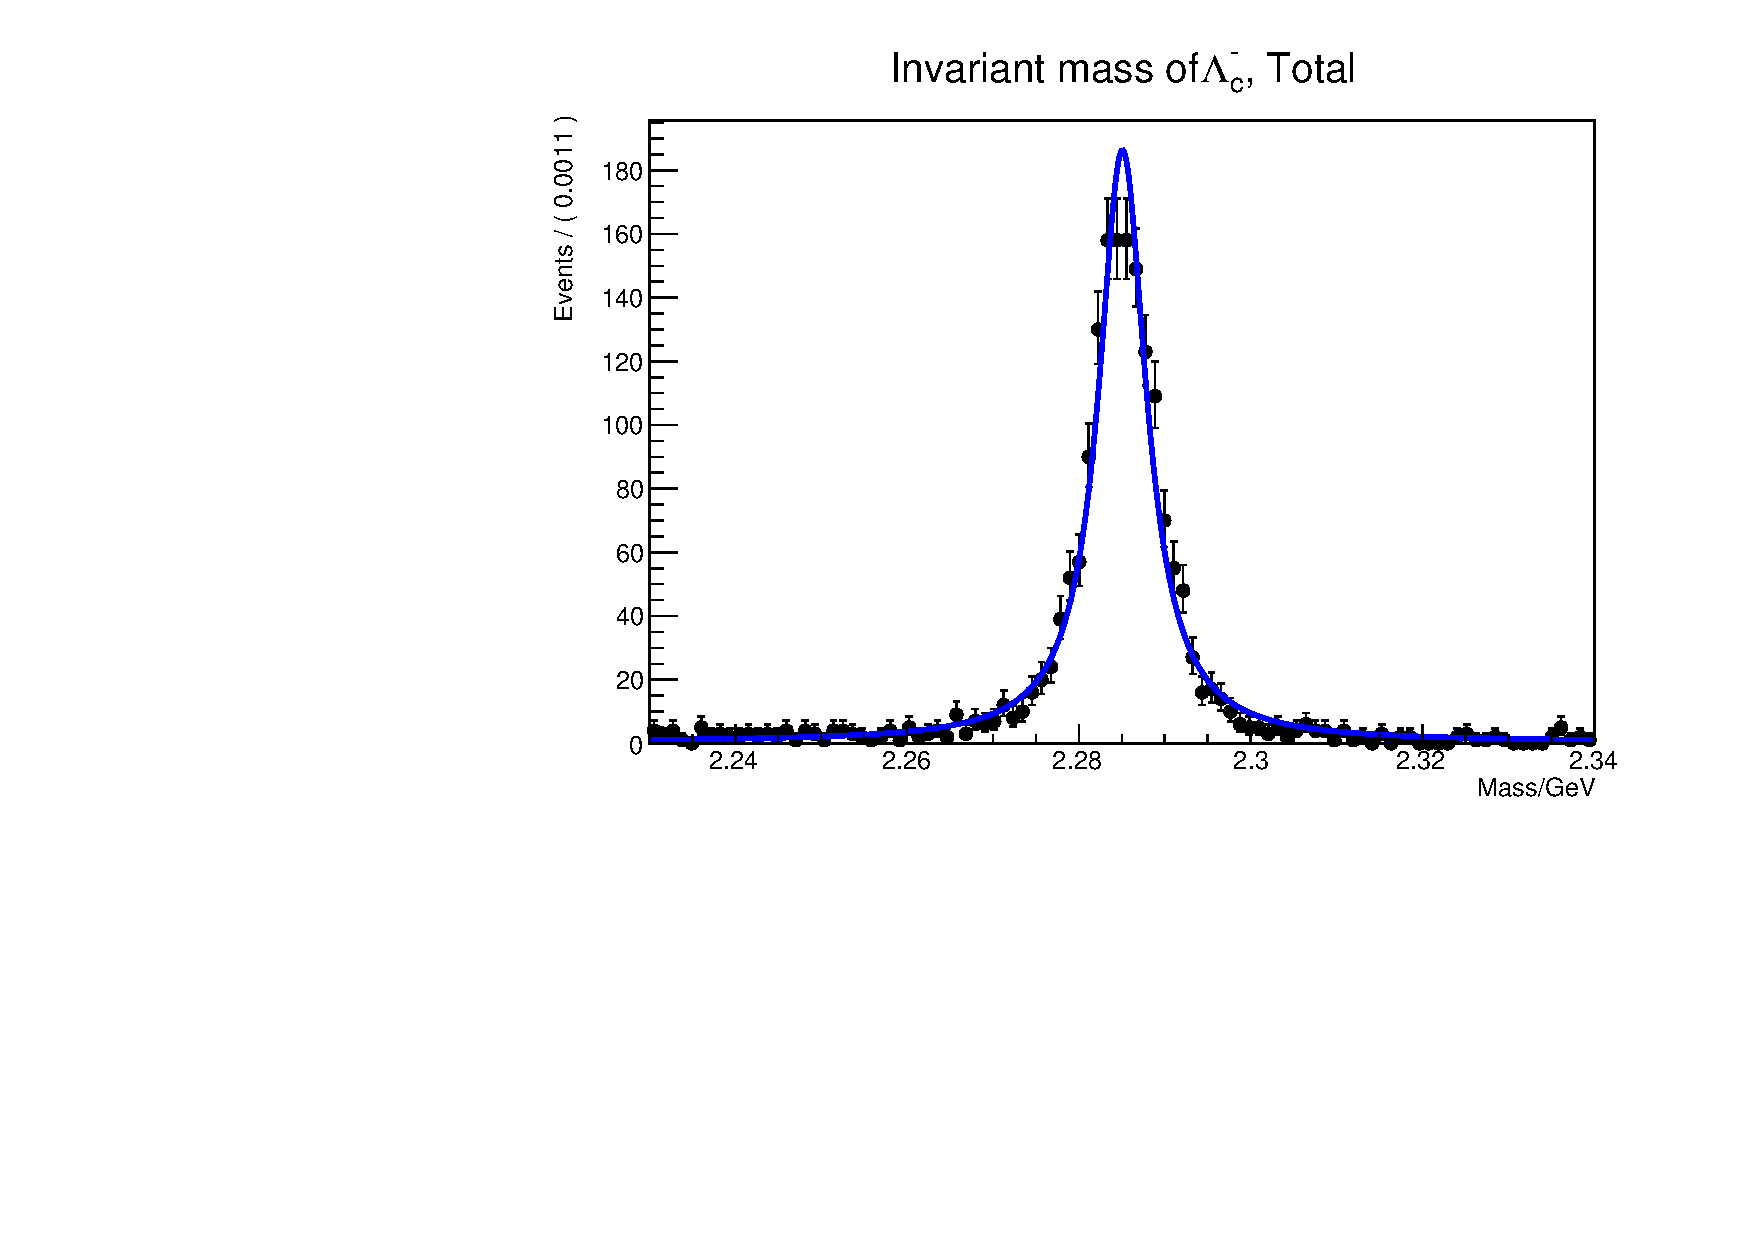
\includegraphics[width = 0.75\textwidth]{Overallim.pdf}
        \caption{Reconstructed invariant mass from MC sample, by $\bar{p} K^0_S$ and $\bar{p} K^+ \pi^-$}
        \label{fig: mBC data}
      \end{figure}
\end{frame}

\begin{frame}
    When reconstructed by $\bar{p} K^0_S$ and $\bar{p} K^+ \pi^-$ seperately:
    \begin{figure}
        \centering
        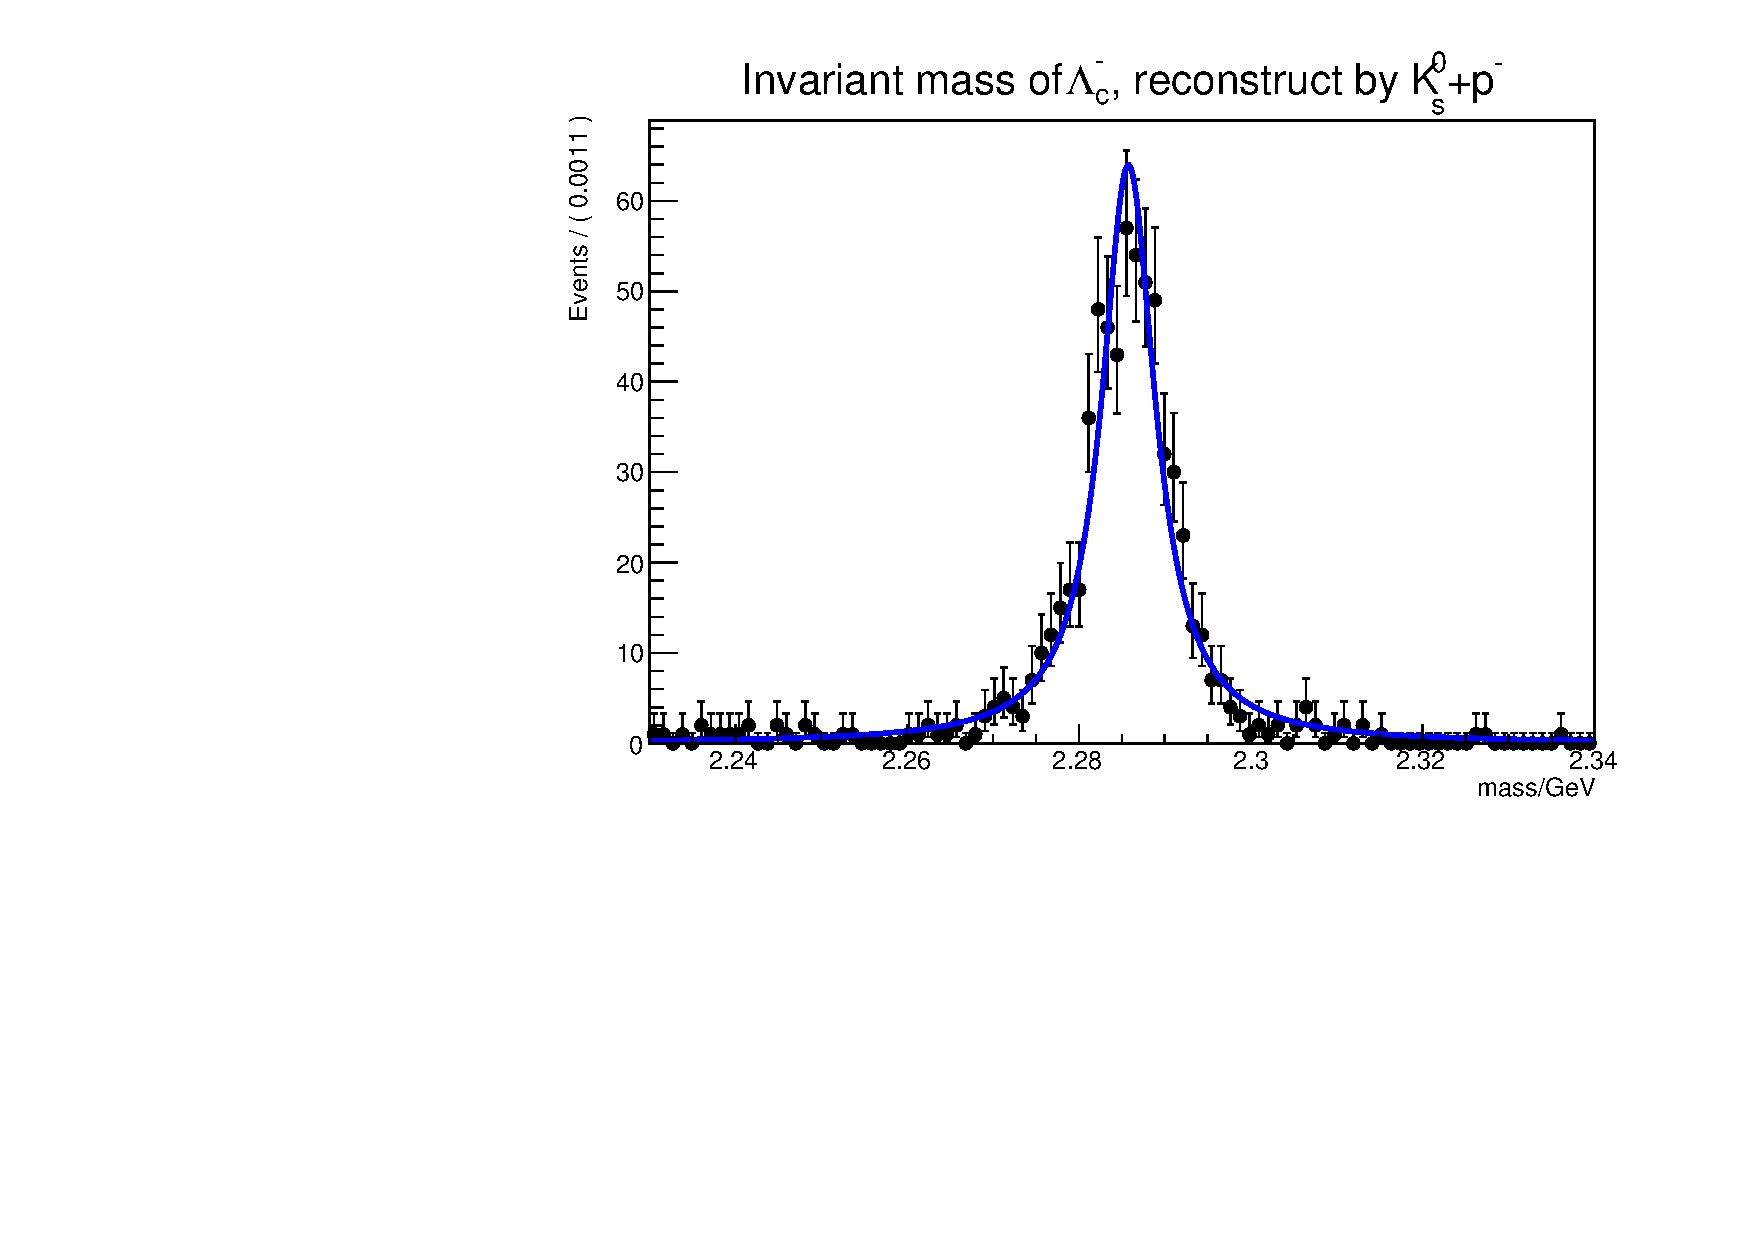
\includegraphics[width = 0.75\textwidth]{k0p.pdf}
        \caption{Reconstructed invariant mass from MC sample, by $\bar{p} K^0_S$ }
        \label{fig: mBC data}
      \end{figure}
\end{frame}

\begin{frame}
    When reconstructed by $\bar{p} K^0_S$ and $\bar{p} K^+ \pi^-$ seperately:
    \begin{figure}
        \centering
        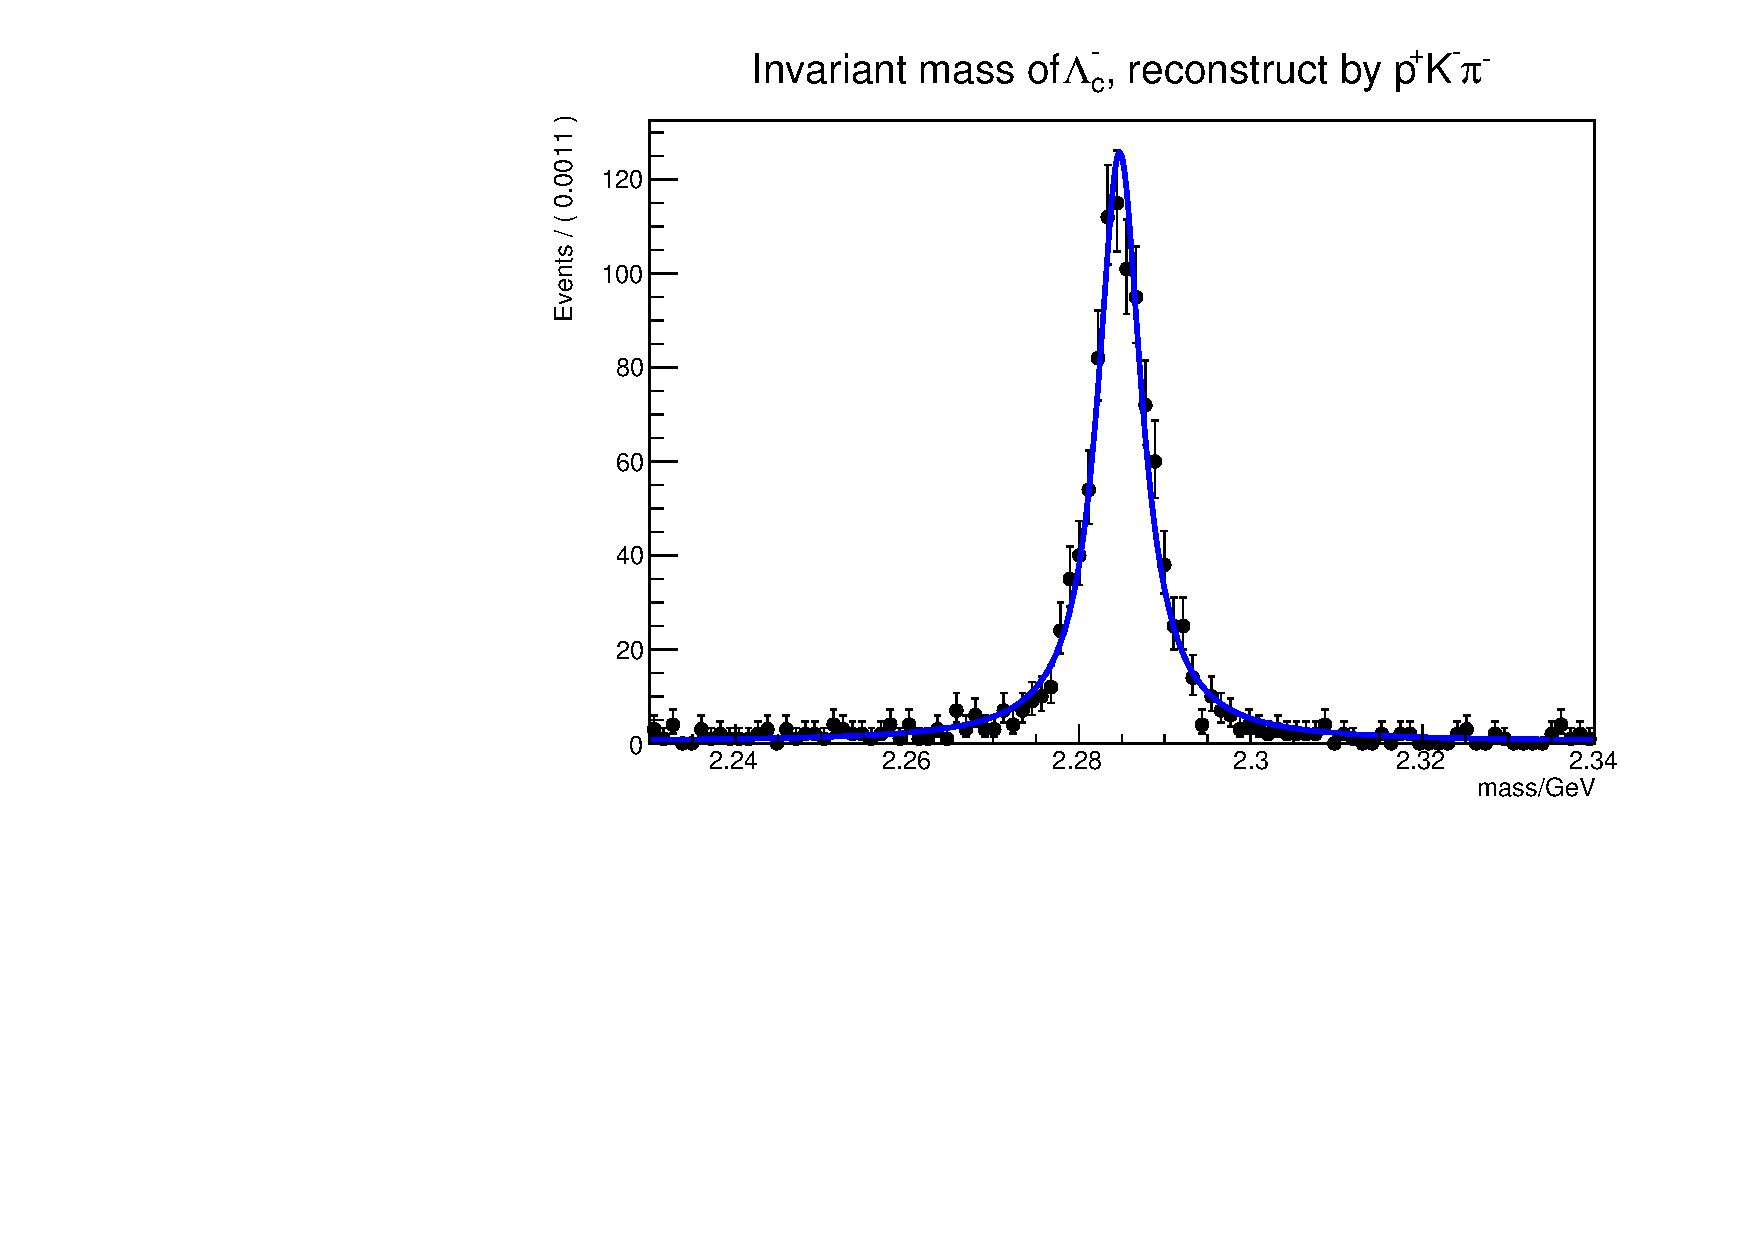
\includegraphics[width = 0.75\textwidth]{unnamed.pdf}
        \caption{Reconstructed invariant mass from MC sample, by $\bar{p} K^+ \pi^-$ }
        \label{fig: mBC data}
      \end{figure}
\end{frame}

\begin{frame}
    To suppress combinatorial backgrounds, $\Delta E \equiv E_{\bar{\Lambda}_c^-} -E_{\rm beam}$ should in $(-3\sigma,3\sigma)$ and $M_{\rm BC}=\sqrt{E_{\rm beam}^2/c^4-|\vec{p}_{\bar{\Lambda}_c^-}|^2/c^2}$ should satisify $2.282 <M_{\rm BC}<2.300~{\rm GeV}/c^2$\\
    \vspace{0.2in}
    After the selection, the effiency fails to $45\%$. Less than the effiency listed in the article:
    \begin{table}[ht]
        \centering
        \caption{ Summary of $\Delta E$  requirements, detection efficiencies and  ST yields for the different tag modes.(Copied from article)}
        \begin{tabular}{lccc}
        \hline
        \hline
        Tag {mode} & $\Delta E$ (MeV) & Efficiency (\%) & Yield\\
        \hline
        $\bar{\Lambda}_c^- \rightarrow \bar{p} K^0_S    $ & $(-21, 19)$ & $56.5\pm0.3$ & $1214\pm36$  \\
        $\bar{\Lambda}_c^- \rightarrow \bar{p} K^+ \pi^-$ & $(-20, 16)$ & $50.1\pm0.1$ & $6092\pm82$  \\
        \hline
        \hline
        \end{tabular}
        \label{table: summary of ST data}
    \end{table}
\end{frame}

\section{PID}
\begin{frame}
    
\end{frame}

\section{References}
\begin{frame}[allowframebreaks]
    \bibliography{ref}
\end{frame}

\end{document}